\documentclass{beamer}
\mode<presentation>
\usepackage[english]{babel}
\usepackage[utf8]{inputenc}

\usepackage {amsmath,amssymb,amsthm,latexsym,tikz,pgfplots,framed,bbm,comment,graphicx,tabularx,subfig}
\graphicspath{ {img/} }

\usetheme {Frankfurt}
\usecolortheme {default}

%----- page numbering
\beamertemplatenavigationsymbolsempty
\setbeamerfont{page number in head/foot}{size=\large}
\setbeamertemplate{footline}[frame number]

%----- definitions
\def \R{{\mathbb{R}}}
\def \P{{\mathbb{P}}}
\def \E{{\mathbb{E}}}

%----- title page and document
\title{Connectivity analysis of device-to-device cellular network using stochastic geometry}
\author{Gulomov Saidkhuja\\14M54020}
\institute{Department of Mathematical and Computing Sciences\\Tokyo Institute Of Technology}
\begin{document}
  \frame {\titlepage}
  \begin {frame}
  \frametitle {Abstract}
  \begin{itemize}
    \item Device-to-device (D2D) enables direct communication between nearby mobiles;
    \item D2D improves spectrum utilization, energy efficiency, coverage and overall throughput;
    \item Thesis considers D2D cellular network in comparison with the traditional cellular network;
    \item Model consists of independent homogeneous Poisson point processes with contact distance probability and noise-limited environment;
    \item Analytical way of calculating performance is developed;
    \item Using analytical results, numerical experiments are carried out and results are displayed.
  \end{itemize}
\end {frame}

  \begin {frame}
    \frametitle {Table of contents}
    \tableofcontents
  \end {frame}
  \section {Introduction}

\begin {frame}
  \frametitle {Device-to-device communication}
  \begin{minipage}{0.45\textwidth}
	\begin{itemize}
	  \item Growing demands of network capacity has led to evolution of networks from 1G to 5G;
	  \item Device-to-device (D2D) communication becomes an effective facilitator of the upcoming high data rate; 
	\end{itemize}
  \end{minipage}
  \begin{minipage}{0.4\textwidth}
    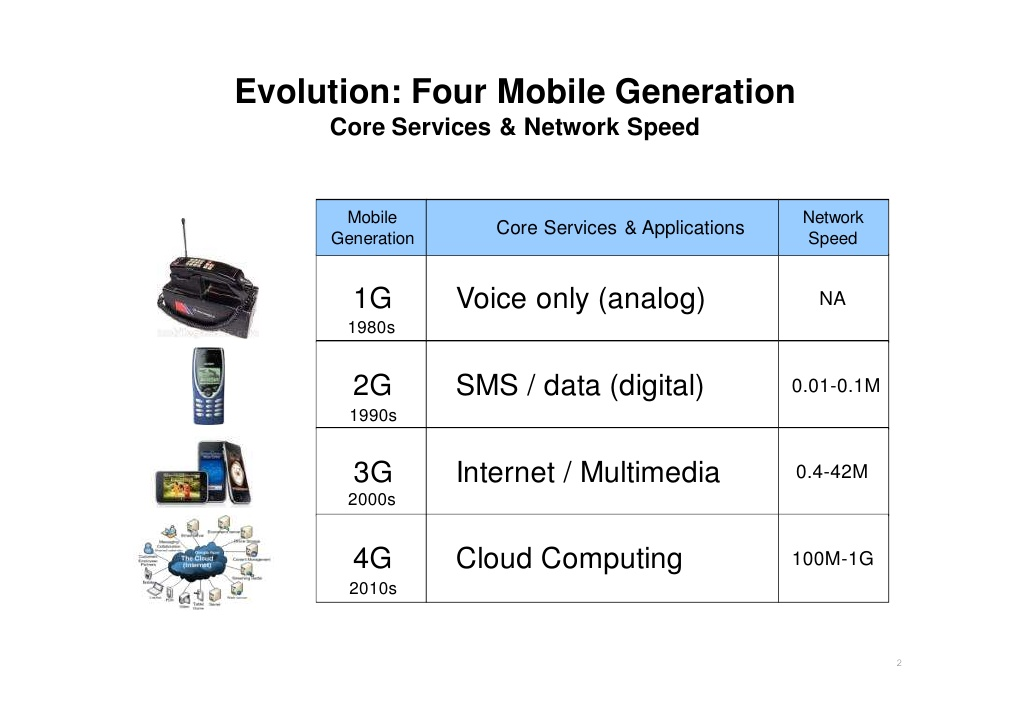
\includegraphics[scale=0.2]{net_evol}
  \end{minipage}
\end {frame}

\begin {frame}
  \frametitle {Overview of the existing studies on device-to-device communication}
  Device-to-device communication is classified into 2 major groups:
  \begin {enumerate}
    \item D2D sharing cellular spectrum, {\it a.k.a {\bf inband}};
    \begin{itemize}
      \item spectrum utilization;
      \item power efficiency;
      \item cellular coverage
    \end{itemize}
    \begin{itemize}
      \item interference.
    \end{itemize}
    \item D2D exploits unlicensed spectrum, {\it a.k.a {\bf outband}};
    \begin{itemize}
      \item video transmission;
      \item average file transfer delay.
    \end{itemize}
  \end{enumerate}
\end {frame}

  \section {Problem}

\begin {frame}
  \frametitle {System model}
  \begin{itemize}
    \item 2 stationery independent homogeneous PPPs of base stations and mobile users \((\Phi_b, \Phi_u)\);
    \item Given parameters \((\lambda_b,P_b,N_b,\beta_b,\Theta_b),(\lambda_u,P_u,N_u,\beta_u,\Theta_u)\);
    \item Rayleigh fading with mean 1;
    \item Noise-limited environment;
    \item Receiver at the origin of \(\R^2\), nearest BS at \(B_{nst}\);
    \item Distance to the nearest BS as \(d_b\), to the nearest D2D node - \(d_u\)
  \end{itemize}
\end {frame}

\begin {frame}
  \frametitle {Performance evaluation}
\par The key performance characteristics that the paper considers is Signal-to-Noise ratio (SNR).
\[SNR_{nf}=\frac {S} {N}=\frac {Pd^{-\beta}} {N},\]
for channel without fading; and
\[SNR_f=\frac {Phd^{-\beta}} {N},\]
for channel with fading where $h$ - random variable that follows an exponential distribution with mean $1/\mu$ which we denote as $h\sim \exp(\mu)$.
\end {frame}

\section {Results}

\begin {frame}
  \frametitle{Performance evaluation}
The purpose of the thesis is to consider the following probabilities:
\begin{equation}
p_{nf}=\P\Big[SNR_{nf}\ge\Theta\Big]=\P\Big[d\le\big(\frac{P}{N\Theta}\big)^{1/\beta}\Big],
\end{equation}
and:
\begin{equation}
p_{f}=\P\Big[SNR_f\ge\Theta\Big]=\P\Big[h\ge\frac{Nd^{\beta}\Theta}{p}\Big].
\end{equation}
Considering (1) for BS and D2D node, we get:
\[\P\Big[d_b\le R_1\Big]\text{, where }R_1=\Big(\frac {P_b} {N_b\Theta_b}\Big)^{1/\beta_b}\]
\[\P\Big[d_u\le R_2\Big]\text{, where }R_2=\Big(\frac {P_u} {N_u\Theta_u}\Big)^{1/\beta_u}\]
Scenarios under consideration:
\begin{enumerate}
  \item \(d_b\le R_1\)--direct cellular connection;
  \item \(R_1<d_b\le R_1+R_2\)--single D2D relay connection.
\end{enumerate}
\end{frame}

\begin{frame}
  \frametitle {Direct cellular connection}
  \begin {block} {Cellular connection with non-fading channel}
    \[p_{nf}^{cel}=1-\exp(-\lambda_b\pi R_1^2)\]
  \end {block}
  \begin{minipage}{.65\textwidth}
    {\it Idea:} Using (1) and \(R_1\) we get:
    \[\P[d_b\le R_1]=1-\P[\Phi_b(b(o,R_1))=0]\]
  \end{minipage}
  \begin{minipage}{.3\textwidth}
        \begin{tikzpicture}[scale=.5]
        \begin{axis}[
            xmin=-3,xmax=3,
            ymin=-3,ymax=3,
            extra x ticks={-1,1,-2,2,-3,3},
            extra y ticks={-1,1,-2,2,-3,3},
            extra tick style={grid=both},
        ]
        \draw[red] \pgfextra{
          \pgfpathcircle{\pgfplotspointaxisxy{0}{0}}{2.5cm}
          };
        \node[inner sep=0pt] (receiver) at (3.4cm,2.9cm)
            {
\includegraphics[width=.1\textwidth]{phone.jpg}};
        \node[inner sep=0pt] (receiver) at (4.4cm,0.9cm)
            {
\includegraphics[width=.3\textwidth]{bs.png}};
        \end{axis}
    \end{tikzpicture}

  \end{minipage}
\end{frame}

\begin{frame}
  \frametitle{Single D2D relay link connection}
  \begin {block} {Single D2D relay connection with non-fading channel}
  \[p_{nf}^{s-hop}=2\lambda_b\pi\int_{R_1}^{R_1+R_2}r\exp(-\lambda_b\pi r^2)(1-\exp(-\lambda_u|D(r)|))dr,\]
  where $|D(r)|=R_2^2 \cos^{-1}\Big(\frac {r^2 + R_2^2 - R_1^2} {2rR_2}\Big)+R_1^2\cos^{-1}\Big(\frac {r^2 + R_1^2 - R_2^2} {2rR_1}\Big)-\frac {1} {2}\sqrt{(R_2+R_1-r)(r+R_2-R_1)(r-R_2+R_1)(r+R_1+R_2)}$.
  \end {block}
\end{frame}

\begin{frame}
  \frametitle{Single D2D relay link connection}
  \begin {minipage}{0.65\textwidth}
{\it Idea:} We consider the event \(C=\Big[\Phi_u\big(b(o,R_2)\cap b(B_{nst},R_1)\big)\ge1,d_b\in(R_1;R_1+R_2]\Big]\). 
We then derive a PDF of (1) for case of a mobile user \(f_{d_b}(r)=\frac{d}{dr}(\P(d_b\le r))=2\lambda_b\pi re^{-\lambda_b\pi r^2}\). 
We use the conditioning on the nearest BS to be at distance \(r,\quad d_b=r\) and compute the integral:
\[\int_{R_1}^{R_1+R_2}f_{d_u}(r)\P\Big(\Phi_u\big(b(o,R_2)\cap b(B_{nst},R_1)\ge1\big)\Big|d_b=r\Big)\]
  \end{minipage}
  \begin{minipage}{0.3\textwidth}
        \begin{tikzpicture}[scale=0.5]
        \begin{axis}[
            xmin=-3,xmax=10,
            ymin=-3,ymax=10,
            extra x ticks={0,-1,1,-2,2,-3,3,-4,4},
            extra y ticks={0,-1,1,-2,2,-3,3,-4,4},
            extra tick style={axis equal=true,grid=both},
        ]
		\draw[red,dashed] \pgfextra{
		  \pgfpathcircle{\pgfplotspointaxisxy{0}{0}}{2.5cm}
		};
		\draw[red,dashed] \pgfextra{
		  \pgfpathcircle{\pgfplotspointaxisxy{4}{4}}{2.5cm}
		};
		\draw[blue] \pgfextra{
		  \pgfpathcircle{\pgfplotspointaxisxy{0}{0}}{1cm}
		};
		\addplot graphics[xmin=-0.2,xmax=0.2,ymin=-0.4,ymax=0.4]{phone.jpg};
		\addplot graphics[xmin=0.8,xmax=1.2,ymin=0.6,ymax=1.4]{phone.jpg};
		\addplot graphics[xmin=3.6,xmax=4.4,ymin=3.6,ymax=4.6]{bs.png};
        \end{axis}
    \end{tikzpicture}

  \end{minipage}
\end {frame}

\begin {frame}
  \frametitle {Cellular connection with fading effect.}
  \begin {block} {Cellular connection with fading in the channel}
  \[p_{f}^{cel}=2\lambda_b\pi\int_{r>0}\exp\Big(-\frac {\mu \Theta_b N_b r^{\beta_b}} {P_b}\Big)r\exp(-\lambda_b\pi r^2)dr\]
  \end {block}
{\it Idea:} We condition on the nearest BS to be at distance \(r\), and using (2) we consider the following probability:
\[\P\Big[h\ge\frac{N_bd^{\beta_b}\Theta_b}{P_b}\Big|d_b=r\Big]\]
We then use the PDF of \(d_b\) -- \(f_{d_b}(r)\) and compute the integral:
\[\int_{r>0}f_{d_b}(r)\P\Big[h\ge\frac{N_br^{\beta_b}\Theta_b}{P_b}\Big]\]
\end {frame}

  \section{Numerical experiments}
\begin{frame}
\frametitle{Testing environment}
Simulations were conducted for cases:
\begin{enumerate}
    \item direct cellular connection (without fading);
    \item direct cellular connection (with fading);
	\item direct cellular connection or single D2D relay link (without fading);
\end{enumerate}
The value of the precision used during the numerical integration is $10^{-3}$.
\end{frame}

\begin{frame}
  \frametitle{Initial testing parameters}
The following data was used as a baseline sample for experiments:

\begin{center}
    \begin{tabular}{ | l | p{3cm} | }
	  \hline
	  Symbol & Simulation value \\
	  \hline
	  ${P_u}$ & 23 dBm\\
	  ${P_b}$ & 46 dBm+14 dBi\\
	  ${\lambda_u}$ & ${5\times 10^{-5}}$\\
	  ${\lambda_b}$ & $10^{-6}$\\
	  ${N_u}$ & -105 dBm\\
	  ${N_b}$ & -99 dBm\\
	  ${\Theta_u}$ & 10 dB\\
	  ${\Theta _b}$ & 5 dB\\
	  ${\beta_u}$ & 3.68\\
	  ${\beta_b}$ & 3.52\\
	  \hline
	\end{tabular}
\end{center}
\end{frame}

\begin{frame}
\frametitle{Testing scenarios.}
Parameters left to be constant:
\begin{itemize}
  \item transmission power;
  \item thermal noise;
  \item service threshold.
\end{itemize}
Parameters being tested:
\begin{itemize}
  \item density;
  \item propagation exponents.
\end{itemize}
\end{frame}

\begin{frame}
  \frametitle{Direct cellular connection or single D2D relay link without fading}
  \begin{minipage}{.5\textwidth}
	\begin{figure}[!hb]
		\begin{tikzpicture}[scale=.6]
		  \begin{axis}[xmin=0.00000001,xmax=0.00003,ymin=0.000001,ymax=0.1,zmin=0,zmax=1,legend style={at={(0.5,-0.20)},anchor=north},grid=major,xlabel={\(\lambda_b\), BS density},ylabel={\(\lambda_u\), UE density},zlabel={probability}]
		    \addplot3 table[header=false,y expr=0] {tables_new/d2d_nf_c_ds_prob0.txt};
		    \label {pgfplots:d2d_nf_c_ds_prob0}
		    \addlegendentry {\(\beta_b=3.52\)}
		    \addplot3[surf] table[header=false] {tables_new/d2d_nf_ds_prob0.txt};
		    \label {pgfplots:d2d_nf_ds_prob0}
		    \addlegendentry {\(\beta_b=3.52\)/\(\beta_u=3.68\)}
		    \addplot3 table[header=false,y expr=0] {tables_new/d2d_nf_c_ds_prob1.txt};
		    \label {pgfplots:d2d_nf_c_ds_prob1}
		    \addlegendentry {\(\beta_b=2.7\)}
		    \addplot3[surf] table[header=false] {tables_new/d2d_nf_ds_prob2.txt};
		    \label {pgfplots:d2d_nf_ds_prob2}
		    \addlegendentry {\(\beta_b=2.7\)/\(\beta_u=2.86\)}
		  \end{axis}
		\end{tikzpicture}
	  \caption {}
	\end{figure}
  \end{minipage}
  \qquad
  \begin{minipage}{.4\textwidth}
	{\bf \(\beta_b=3.52\)/\(\beta_u=3.68\):}
    \resizebox{\textwidth}{!}{
	\begin{tabular}{|c|c|c|}
	\(\lambda_b\) & \(\lambda_u\) & \(\P\) \\ \hline
	0.00000001 & 0.000001 & 0.008 \\ \hline
	0.00000005 & 0.000010 & 0.039 \\ \hline
	0.00000025 & 0.000100 & 0.178 \\ \hline
	0.00000125 & 0.001000 & 0.626 \\ \hline
	0.00000625 & 0.010000 & 0.993 \\ \hline
	0.00003125 & 0.100000 & 1.000 \\ \hline
	\end{tabular}}
	{\bf \(\beta_b=2.7\)/\(\beta_u=2.86\):}
    \resizebox{\textwidth}{!}{
	\begin{tabular}{|c|c|c|}
	\(\lambda_b\) & \(\lambda_u\) & \(\P\) \\ \hline
	0.00000001 & 0.000001 & 0.290 \\ \hline
	0.00000005 & 0.000010 & 0.819 \\ \hline
	0.00000025 & 0.000100 & 1.000 \\ \hline
	\end{tabular}}
  \end{minipage}
\end{frame}

\begin{frame}
  \frametitle{Direct cellular connection or single D2D relay link without fading}
  \begin{minipage}{.5\textwidth}
	\begin{figure}[!hb]
		\begin{tikzpicture}[scale=.6]
		  \begin{axis}[mesh/ordering=y varies,xmin=0.00000001,xmax=0.0008,ymin=0.01,ymax=100,zmin=0,zmax=1,legend style={at={(0.5,-0.20)},anchor=north},grid=major,xlabel={\(\lambda_b\), BS density},ylabel={\(\lambda_u\), UE density},zlabel={probability}]
		    \addplot3 table[header=false,y expr=0] {tables_new/d2d_nf_c_ds_prob2.txt};
		    \label {pgfplots:d2d_nf_c_ds_prob2}
		    \addlegendentry {\(\beta_b=6\)/\(\beta_u=6\)}
		    \addplot3[surf] table[header=false] {tables_new/d2d_nf_ds_prob3.txt};
		    \label {pgfplots:d2d_nf_ds_prob3}
		    \addlegendentry {\(\beta_b=6\)/\(\beta_u=6\)}
		  \end{axis}
		\end{tikzpicture}
	  \caption {}
	\end{figure}
  \end{minipage}
  \qquad
  \begin{minipage}{.4\textwidth}
	{\bf \(\beta_b=6\)/\(\beta_u=6\):}
    \resizebox{\textwidth}{!}{
	\begin{tabular}{|c|c|c|}
	\(\lambda_b\) & \(\lambda_u\) & \(\P\) \\ \hline
	0.00000025 & 0.000100 & 0.001 \\ \hline
	0.00000125 & 0.001000 & 0.006 \\ \hline
	0.00000625 & 0.010000 & 0.029 \\ \hline
	0.00003125 & 0.100000 & 0.139 \\ \hline
	0.00015625 & 1.000000 & 0.595 \\ \hline
	0.00078125 & 10.000000 & 0.997 \\ \hline
	0.00390625 & 100.000000 & 1.000 \\ \hline
	\end{tabular}}
	{\bf \(\beta_b=6\):}
    \resizebox{3cm}{!}{
	\begin{tabular}{|c|c|}
	\(\lambda_b\) & \(\P\) \\ \hline
	0.00000025 & 0.001 \\ \hline
	0.00000125 & 0.006 \\ \hline
	0.00000625 & 0.028 \\ \hline
	0.00003125 & 0.134 \\ \hline
	0.00015625 & 0.514 \\ \hline
	0.00078125 & 0.973 \\ \hline
	\end{tabular}}
  \end{minipage}
\end{frame}

  \section{Conclusion}

\begin {frame}
\frametitle{General results.}
\begin{itemize}
  \item Derivation of analytical formulas for performance evaluation;
  \item Numerical experiments are carried out;
  \item D2D enabled cellular network becomes useful when the signal propagation is seriously obstructed;
  \item D2D enabled cellular network yields good performance when the ratio of the number of base stations to the number of mobile users is around \(1/10,000\).
\end{itemize}
\end {frame}

\begin{frame}
\frametitle{Future work}
\begin{itemize}
  \item Consideraion of \(n\)--D2D relay links in both non-fading channel and channel with fading;
  \item Interference modelling;
  \item Additional relaying layer can be added into the model and performance evaluation is also possible (like in project 'OneWeb').
\end{itemize}
\end{frame}

\begin{frame}
\frametitle{Acknowledgements}
Student Gulomov Saidkhuja would like to express his deep gratitude to prof. Naoto Miyoshi for his extensive support and help during the preparation of the work.
\end{frame}

\end{document}
